\section*{Problema 1}

\textbf{Usemos la distancia de Kullback-Leibler para T-SNE. En el caso discreto, la definición de la distancia de Kullback-Leibler es:}

\begin{equation*}
    d(P^1,P^2) = \sum_i P^1_i \log \left (\frac{P^1_i}{P^2_i} \right )
\end{equation*}

\begin{itemize}
    \item Calcula $d(P^1,P^2)$ si $P^1\sim Bern(\theta_1)$ y $P^2 \sim Bern(\theta_2)$.
    \item Grafica $d(P^1 , P^2)$ como función de $\theta_2$ con $\theta_1$ fija, y verifica que efectivamente mide de alguna manera la disimilitud entre $P^1$ y $P^2$ .
\end{itemize}

Se tiene que

\begin{equation*}
    P(\theta) = \theta^x (1-\theta)^{1-x}
\end{equation*}

Calculando $ \log \left (\frac{P^1_i}{P^2_i} \right )$, se obtiene que:

\begin{align*}
    \log \left (\frac{P^1_i}{P^2_i} \right ) & = \log \left (\frac{\theta_1^x (1-\theta_1)^{1-x}}{\theta_2^x (1-\theta_2)^{1-x}} \right )                   \\
                                             & = \log \left (\theta_1^x (1-\theta_1)^{1-x} \right ) - \log \left (\theta_2^x (1-\theta_2)^{1-x}\right )     \\
                                             & = x \log (\theta_1) + (1-x) \log (1-\theta_1) -x \log (\theta_2) - (1-x) \log (1-\theta_2)                   \\
                                             & = x \left(\log (\theta_1)-\log (\theta_2)\right) + (1-x) \left (\log (1-\theta_1)-\log (1-\theta_2) \right )
\end{align*}

Entonces, la distancia de Kullback-Leibler para dos distribuciones de Bernoulli es la siguiente:

\begin{align*}
    d(P^1,P^2) & = \sum_{i=0}^1 \theta_1^i (1-\theta_1)^{1-i}\left [ i \left(\log (\theta_1)-\log (\theta_2)\right) + (1-i) \left (\log (1-\theta_1)-\log (1-\theta_2) \right ) \right ] \\
    d(P^1,P^2) & = (1-\theta_1) \left ( \log (1-\theta_1)- \log (1-\theta_2)\right ) + \theta_1 \left (\log (\theta_1)-\log (\theta_2) \right )
\end{align*}

Por lo tanto, la distancia de Kullback-Leibler para dos distribuciones de Bernoulli se puede calcular como en la ecuación \ref{eq:problema_01}.

\begin{equation}
    d(P^1,P^2)  = (1-\theta_1) \left ( \log (1-\theta_1)- \log (1-\theta_2)\right ) + \theta_1 \left (\log (\theta_1)-\log (\theta_2) \right ) \label{eq:problema_01}
\end{equation}

En la figura se visualiza la ecuación \ref{eq:problema_01} para diferentes valores de $\theta_1$. En esta se ve que la función alcanza un valor mínimo cuando $\theta_1$ y $\theta_2$ son muy semejantes. Por otro lado esta función tiende a infinito cuando los valores tienen una diferencia mayor.

\begin{figure}[H]
    \centering
    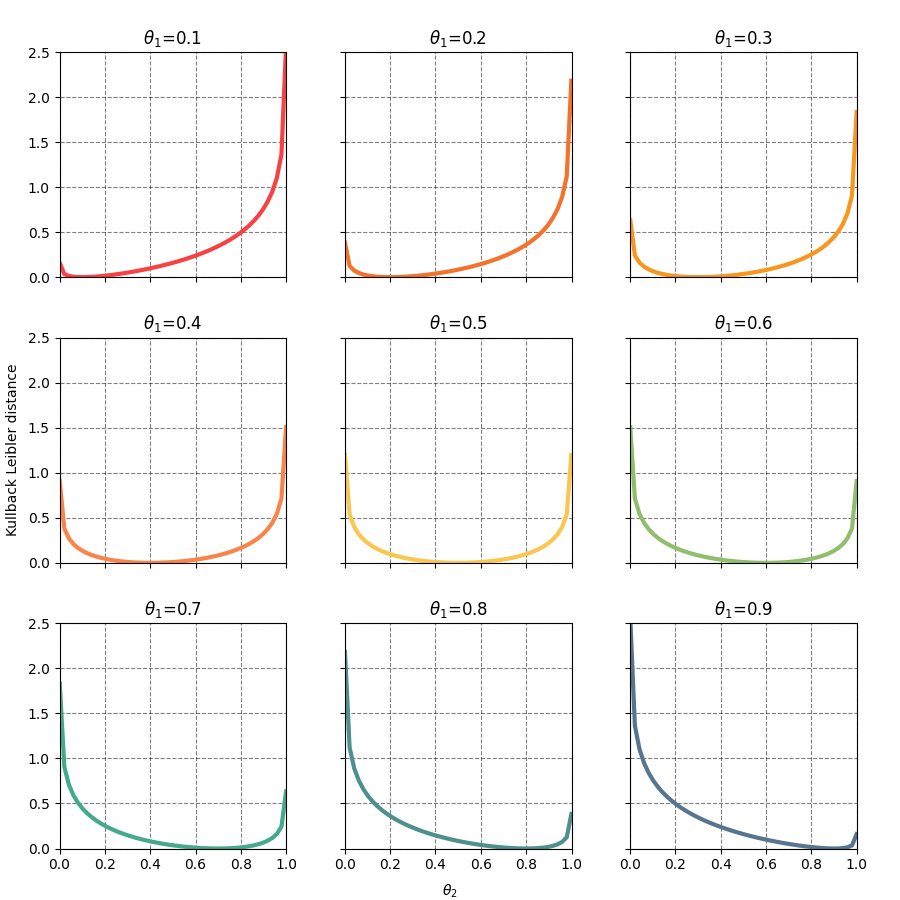
\includegraphics[width=14cm]{Graphics/Kullback.png}
    \caption{Resultados para diferentes valores de $\theta_1$ en la ecuación \ref{eq:problema_01}.}
\end{figure}